
¿Cuál es el perímetro del triángulo de la figura \ref{fig:peri_rect_01}?

% \begin{minipage}[t][][t]{0.3\textwidth}
\begin{figure}[H]
    \centering
    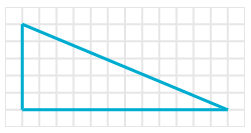
\includegraphics[width=0.2\textwidth]{../images/peri_rect_01.png}
    \caption{}
    \label{fig:peri_rect_01}
\end{figure}
% \end{minipage}\hfill
% \begin{minipage}[t][][t]{0.68\textwidth}
\begin{solutionbox}{16cm}
    \begin{minipage}{0.3\textwidth}
        \begin{figure}[H]
            \centering
            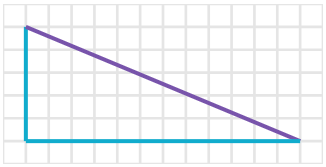
\includegraphics[width=0.6\linewidth]{../images/peri_rect_01a.png}
            \caption{}
            \label{fig:peri_rect_01a}
        \end{figure}
        \begin{figure}[H]
            \centering
            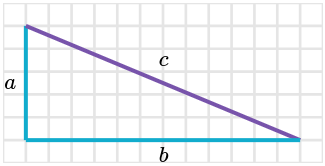
\includegraphics[width=0.6\linewidth]{../images/peri_rect_01b.png}
            \caption{}
            \label{fig:peri_rect_01b}
        \end{figure}
        \begin{figure}[H]
            \centering
            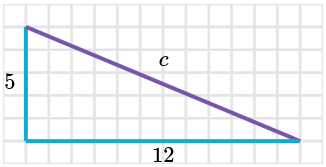
\includegraphics[width=0.6\linewidth]{../images/peri_rect_01c.png}
            \caption{}
            \label{fig:peri_rect_01c}
        \end{figure}
        \begin{figure}[H]
            \centering
            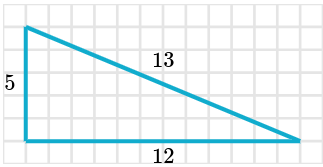
\includegraphics[width=0.6\linewidth]{../images/peri_rect_01d.png}
            \caption{}
            \label{fig:peri_rect_01d}
        \end{figure}
    \end{minipage}\hfill
    \begin{minipage}{0.65\textwidth}
        El perímetro es la distancia alrededor de una figura.
        Cada recta diagonal es la hipotenusa de un triángulo rectángulo (ver Figura \ref{fig:peri_rect_01a}).
        Podemos utilizar el teorema de Pitágoras para encontrar un lado faltante.
        La ecuación del teorema de Pitágoras es:
        \[c^2=a^2+b^2\]
        donde $a$ y $b$ son las longitudes de los catetos, y $c$ es la longitud de la hipotenusa.
        Etiquetemos la Figura del problema con $a$, $b$ y $c$ (ver Figura \ref{fig:peri_rect_01b}).
        Podemos contar los cuadrados para encontrar las longitudes de $a$ y $b$, y luego sustituir esos valores en el teorema de Pitágoras (ver Figura \ref{fig:peri_rect_01c}).
        \begin{align*}
            a^2+b^2  =c^2  & \text{\quad El teorema de Pitágoras}                          \\
            5^2+12^2  =c^2 & \text{\quad Sustituye las longitudes}                         \\
            25 +144 =c^2   & \text{\quad Evalua los cuadrados conocidos}                   \\
            169=c^2        & \text{\quad Sumando }                                         \\
            13=c           & \text{\quad Calculando la raíz en ambos lados de la ecuación} \\
        \end{align*}
        Ahora que conocemos la longitud de la diagonal, podemos encontrar la longitud de los lados faltantes para calcular el perímetro.
        Como los lados faltantes son líneas verticales u horizontales, podemos contar los cuadrados para obtener sus longitudes (ver Figura \ref{fig:peri_rect_01d}).
        \[13+12+5=30\]
        El perímetro del triángulo es 30 unidades.
    \end{minipage}
\end{solutionbox}
% \end{minipage}